\documentclass[xcolor=svgnames]{beamer}
\mode<presentation>
\usetheme{JuanLesPins}
\usecolortheme[named=Teal]{structure}
\setbeamerfont{structure}{shape=\itshape}

\hypersetup{pdfpagemode=FullScreen} % makes your presentation go automatically to full screen

\setbeamertemplate{background canvas}[vertical
shading][bottom=White!40,top=white!30]
\beamertemplatetransparentcovereddynamicmedium
\useoutertheme{infolines}
%\usepackage{beamerthemesplit}
\usepackage{beamerinnerthemerounded}
\usepackage{beamerouterthemesmoothbars}
\usepackage{subfigure}
\usepackage{multicol}
\usepackage{physics}
\usepackage{amsmath,array}
\usepackage{epsfig}
\usepackage{graphicx}
\usepackage{url}
\usepackage{multimedia}
\usepackage{hyperref}
\usepackage{fancybox}
\usepackage{epstopdf}

\definecolor{lg}{rgb}{0.36,0.99,0.82}
\definecolor{dblue}{rgb}{0,0,.5}
\definecolor{dpink}{cmyk}{.2,1,.1,.04}
\definecolor{purple}{rgb}{0.35,0.04,0.64}
\definecolor{borange}{rgb}{1, .388, 0}
\definecolor{dpurple}{rgb}{0.61,0.22,1.00}
\definecolor{purp}{rgb}{0.44,0.00,0.87}
\definecolor{green}{rgb}{0.00,0.44,0.00}

\newtheorem{theo}{Theorem}
\newtheorem{exa}{Example}
\newtheorem{rem}{Remark}

\def\be{\begin{eqnarray}}%%
\def\ee{\end{eqnarray}}%%
\def\ben{\begin{eqnarray*}}%%
\def\een{\end{eqnarray*}}%%
\def\benum{\begin{enumerate}}%%
\def\eenum{\end{enumerate}}%%
\def\cc#1{\{#1\}}
\def\pp#1{\|#1\|}
\def\ld{\lambda}
\def\l{\leqq}
\def\le{\leqslant}
\def\leq{\leqslant}
\def\geq{\geqslant}
\def\ge{\geqslant}
\def\la{\langle}
\def\ra{\rangle}
\def\Strl{\mathop{\rm Strl}}
\def\eps{\epsilon}
\def\vep{\varepsilon}
\def\rint{\mathop{\rm int}}
\def\bx{\bar{x}}
\def\sx{{x^{\star}}}
\def\bR{\bar{R}}
\def\vsi{\varsigma}
\def\rmint{{\rm int}\,}
\def\ds{\displaystyle}
\newcommand{\norm}[1]{\left\Vert#1\right\Vert}
\newcommand{\tens}[1]{
  \mathbin{\mathop{\otimes}\limits_{#1}}}
\linespread{1.1}
\let\conjugatet\overline

\def\CC{\mathbb{C}}
\def\RR{\mathbb{R}}
\def\MM{\mathbb{M}}
\def\NN{\mathbb{N}}
\def\calL{\mathcal{L}}
\def\calM{\mathcal{M}}
\def\rmint{{\rm int\,}}
\def\cT{\mathcal{T}}
\def\cL{\mathcal{L}}
\def\tau{\cT}
\def\Cl{{cl}\,}
\def\rmint{{\rm int}\,}
\def\disp{\displaystyle}

%***********************************************************
\newcommand{\lr}{\left(}
\newcommand{\rr}{\right)}
\newcommand{\lek}{\left[}
\newcommand{\rek}{\right]}
\newcommand{\lge}{\left\{ }
\newcommand{\rge}{\right\} }
\newcommand{\lb}{\left| }
\newcommand{\rb}{\right| }
\newcommand{\lbl}{\left| }
\newcommand{\rbl}{\right| }
%\newcommand{\ra}{\rangle }
%\newcommand{\la}{\langle }
\newcommand{\es}{\emptyset}
\newcommand{\fa}{\forall}
%\newcommand{\ld}{\lambda}
\newcommand{\real}{\mathbb{R}}
%\newcommand{\norm}[1]{\left\Vert#1\right\Vert}
%\newcommand{\eps}{\epsilon}
\newcommand{\del}{\partial}
\newcommand{\seq}[1]{\left<#1\right>}
%\newtheorem{theorem}{\Large{Theorem}}
\newtheorem{deff}{\Large{Definition}}
\newtheorem{proposition}{\bf Proposition}
%\newtheorem{lemma}{\bf Lemma}
%\newtheorem{example}{\bf Example}
%\newcommand{\lr}{\longrightarrow}
\newcommand{\Ll}{\longleftarrow}
%\newcommand{\ra}{\rightarrow}
%\newcommand{\la}{\leftarrow}
\newcommand{\Lra}{\Leftrightarrow}
\newcommand{\da}{\downarrow}
%\newcommand{\del}{\partial}
\newcommand{\ol}{\overline}
\newcommand{\ul}{\underline}
%\newcommand{\ds}{\displaystyle}
%\newcommand{\fa}{\forall}
\newcommand{\nn}{\nonumber}
\newcommand{\nd}{\noindent}
\newcommand{\imply}{\Rightarrow}
\newcommand{\R}{\mathbb{R}}
\newcommand{\N}{\mathbb{N}}
\newcommand{\h}{\mathbb{H}}
\newcommand{\Z}{\mathbb{Z}}
\newcommand{\B}{\mathcal{B}}
\def\CC{\mathbb{C}}
\def\RR{\mathbb{R}}
\def\MM{\mathbb{M}}
\def\NN{\mathbb{N}}
\def\calL{\mathcal{L}}
\def\calM{\mathcal{M}}
\def\rmint{{\rm int\,}}
\def\cT{\mathcal{T}}
\def\cL{\mathcal{L}}
\def\tau{\cT}
\def\Cl{{cl}\,}
\def\rmint{{\rm int}\,}
\def\disp{\displaystyle}
\def\ds{\displaystyle}
\def\bR{\bar{R}}
%***********************************************************


\title{Universal Quantum Computation using Discrete Time Quantum Walk}

\author[MTP Presentation]{MTP Presentation\\[0.5em]
{\scriptsize{By}}\\
[0.5em] Mukesh Bhati \\
(2013MT60604)\\
[0.5em]
{\scriptsize{Under the Supervision of }}\\
[0.5em] Prof. Shravan Kumar\\[2em]}


\institute[] {\scriptsize{Indian Institute of Technology\\  Delhi \\
[0.7em] }}

\date[July, 2018]{}

\begin{document}
\frame{\titlepage}


\begin{frame}
\frametitle{Outline of the presentation}
\begin{enumerate}
%\item Introduction.
\item Introduction.
\item Quantum Computation.
\item Discrete Time Quantum Walk.
\item Quantum Computation using DTQW.
\item Conclusion.
\end{enumerate}
\end{frame}

\begin{frame}\frametitle{Introduction}
\begin{itemize}
\item \textbf{What is Quantum Computing? : } Study of information processing tasks accomplished using quantum mechanical systems.\\
Quantum Physics + Computer Science + Information theory $\imply$ Quantum   Computing
\item \textbf{Why Quantum Computation? }
\begin{enumerate}
\item To speed-up Computation.
\item Reducing Cheap size.
\item Can do what classical do(almost).
\end{enumerate}
\item \textbf{Classical vs Quantum Information}
\end{itemize}

\end{frame}

\begin{frame}
\frametitle{\textbf{Introduction to Quantum Mechanics}}
\begin{itemize}
\item \textbf{Notations :}
\begin{enumerate}\\
[0.5em]
\item \textbf{ket :}
\begin{center}
    $\ket{v} &= \begin{pmatrix}
           a_{1} \\
           a_{2} \\
           \vdots \\
           a_{m}
         \end{pmatrix}$
  \end{center}
\item \textbf{bra :}
Conjugate transpose of $\ket{v}$
\begin{align}
\bra{v} &= \begin{pmatrix}
           \conjugatet{a_{1}} & \conjugatet{a_{2}} & \hdots \conjugatet{a_{m}}
         \end{pmatrix}
\end{align}
\end{enumerate}
\item \textbf{Inner Product :} $(.,.) : V \cross V \rightarrow \mathbb{C}$,
$$\braket{u}{v} = \sum_{i=1}^{n}\conjugatet{u_i} v_i.$$
\end{itemize}
\end{frame}

\begin{frame}
\frametitle{\textbf{Tensor Product}}
Let U and V are two Linear space. Let $dim(U) = n$ and $dim(V) = m$. we define $$\tens{} : (u,v) \rightarrow u \tens{} v$$
such that
$$u \tens{} v = \sum c_{i,j}(\ket{\alpha_i}\tens{}\ket{\beta_j})$$
satisfies the following relations:\\
\begin{enumerate}
\item $(\ket{u} + \ket{v}) \tens{} \ket{w} =  \ket{u} \tens{} \ket{w} + \ket{v} \tens{} \ket{w}$ \\
\item $\ket{w} \tens{} (\ket{u} + \ket{v}) = \ket{w} \tens{}  \ket{u} + \ket{w} \tens{} \ket{v}$\\
\item $(a\ket{u}) \tens{} \ket{v} = \ket{u} \tens{} (a\ket{v}) = a(\ket{u} \tens{} \ket{v})$\\
\end{enumerate}
\end{frame}

\begin{frame}{Unitary Operator}
Let U be a linear Operator then we called it a Unitary Operator if
\begin{center}
$U^{*}U=\mathbb{I}$
\end{center}
The tensor product $U_1 \tens{} U_2$ is a unitary Operator of the space $X_1 \tens{} X_2$ if $U_1$ and $U_2$ are unitary Operator of $X_1$ and $X_2$ respectively.\\
\vspace{0.5cm}
But direct sum $U_1 \oplus U_2 $ may not be a unitary transformation.
\end{frame}


\begin{frame}{The postulates of Quantum Mechanics}
\begin{itemize}
    \item State Space
    \item Evolution 
    \item Measurement
    \begin{enumerate}
        \item Measurement operators
        \item $$p(m) = \bra{\Phi|M^{*}M|\ket{\Phi}}$$
        \item after measurement $$ \dfrac{M_m \ket{\Phi}}{\sqrt{\bra{\Phi|M^{*}M|\ket{\Phi}}}}$$
    \end{enumerate}
\end{itemize}
\end{frame}

\begin{frame}{The postulates of Quantum Mechanics}
\begin{itemize}
    \item Superposition : $$\ket{\Phi} = \alpha_1\ket{0} + \alpha_2\ket{0}+ ..... +\alpha_N\ket{N} $$
    \item Composite System
    \item Entanglement : $$\ket{\phi} = \dfrac{\ket{00} + \ket{11}}{\sqrt{2}}$$
\end{itemize}
\end{frame}


\begin{frame}{Quantum Computation}
\textbf{Qubit}
\begin{enumerate}
    \item Measurement unit of Information
    \item A unit vector in two-dimensional inner-product space(State Space).
    \item A Qubit is state 
\begin{center}
 $\ket{\phi}$ = \alpha$\ket{0}$ + \beta$\ket{1}$
\end{center}
\end{enumerate}
\end{frame}

\begin{frame}{Quantum Computation}
\textbf{Qubit}
\begin{enumerate}
    \item Measurement in computational basis $$M_0 = \ket{0}\bra{0} \hspace{1cm} M_1 = \ket{1}\bra{1}$$
    \item Measurement in bases other than computational basis
    \begin{enumerate}
        \item Measurement basis : $\ket{+} = \dfrac{\ket{0}+\ket{1}}{\sqrt{2}}$ , $\ket{-} = \dfrac{\ket{0}-\ket{1}}{\sqrt{2}}$
        
    \end{enumerate}
\end{enumerate}
\end{frame}

\begin{frame}{Quantum Computation}
\textbf{Multiple Qubit System}
\begin{enumerate}
    \item n-qubit system $V = V_{n-1} \tens{} \hdots \tens{} V_1 \tens{} V_0$, where $V_i(0 \leq i \leq n-1) $
    \item Projective Measurement in multiple Qubit system
    \begin{enumerate}
        \item $P_k : V \rightarrow V_k$ $$P_k = \ket{k}\bra{k}$$
    \end{enumerate}
\end{enumerate}
\end{frame}


\begin{frame}{Quantum Computation}
\textbf{No Cloning Theorem}\\
\textbf{Theorem 5.1.3.1 :} An unknown state can not be clone using any unitary transformation. Namely, there is no unitary transformation U, such that state $\ket{\phi}$, $U(\ket{\phi,0}) = \ket{\phi,\phi}$. No Cloning theorem hold for any Hilbert space.\\
\textbf{Proof :} Let assume that there exist such unitary transformation U and for two different orthogonal state $\ket{\phi}$ and $\ket{\psi}$, $U(\ket{\phi,0}) = \ket{\phi,\phi}$ and $\ket{\psi}$, $U(\ket{\psi,0}) = \ket{\psi,\psi}$. let $\ket{\gamma} = \dfrac{\ket{\phi} + \ket{\psi}}{\sqrt{2}}$. Then $U(\ket{\gamma,0}) = \dfrac{\ket{\phi,\phi} + \ket{\psi,\psi}}{\sqrt{2}} \neq \ket{\gamma,\gamma} = \dfrac{\ket{\phi,\phi} + \ket{\psi,\psi} + \ket{\phi,\psi} + \ket{\psi,\phi}}{2}$.
\end{frame}

\begin{frame}{Quantum Computation}
\textbf{Quantum Gates}
\begin{itemize}
    \item  unitary operator $U: H_{2^n} \rightarrow H_{2^n}$
    \item NOT Gate $$X = \begin{pmatrix}
                               0 & 1\\
                               1 & 0
                        \end{pmatrix} $$
    \item Phase Gate: $$Y = \begin{bmatrix}
                                1  & 0\\
                                0  & -1
                            \end{bmatrix}$$
    \item NOT-Phase Transformation
    $$\mathbb{Z} = \begin{bmatrix}
                     0  & 1\\
                     -1  & 0
                    \end{bmatrix}$$
\end{itemize}
\end{frame}

\begin{frame}{Quantum Computation}
\textbf{Quantum Gates}
\begin{itemize}
    \item  Hadamard Gate $$H = \dfrac{1}{\sqrt{2}}\begin{pmatrix}
           1 & 0\\
           0 & -1
\end{pmatrix}$$
    \item CNOT Gate $$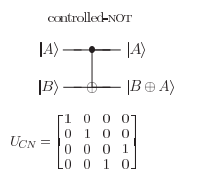
\includegraphics[width = 5cm]{CNOT.png}$$
\end{itemize}
\end{frame}

\begin{frame}{Quantum Walk}
\textbf{Classical Random Walk}
\begin{enumerate}
    \item Guassian Distribution(without factor 2) $$ p(t,n) \simeq \frac{2}{\sqrt{2\pi t}} e^{\frac{-n^{2}}{2t}} $$
    \item Expected Position, $E(n) = 0$.
    \item Standard deviation,  $\sigma = \sqrt{t}$
\end{enumerate}  
\end{frame}

\begin{frame}{Discrete Time Quantum Walk}
\begin{enumerate}
    \item State Space is Hilbert space. $$H_c \tens{} H_p$$ where $H_p$ is Position Space and $H_c$ is Coin Space.
    \item Evolution Operator $$U = S ( H \tens{} I)$$
    \item Generic state $$\ket{\psi} = \sum_{n} \alpha_{n,1}\ket{n,1} + \alpha_{n,0}\ket{n,0}$$
    \item After t time step $$\ket{\psi(t)} = U^t\ket{\psi(0)}$$
\end{enumerate}
\end{frame}

\begin{frame}{Discrete Time Quantum Walk On Line}
    \begin{itemize}
        \item Computational basis of $H_p$ is $$\{\ket{n}: n \in Z\}$$.
        \item $H_c$ is 2 dimensional space with computational basis $$\{\ket{0},\ket{1}\}$$
        \item State Space $$\{\ket{s,n}, s \in {0,1}, n \in Z\}$$
        \item The generic state at time t $$\ket{\psi(t)} = \sum_{s=0}^{1}\sum_{n=-\infty}^{n=\infty}\ket{\psi_{s,t}(t)\ket{s,n}}$$
    \end{itemize}
\end{frame}
\begin{frame}{Discrete Time Quantum Walk On Line}
\begin{itemize}
    \item Probability distribution $$P_n(t) = |\ket{\psi_{0,n}(t)}|^2 + |\ket{\psi_{1,n}(t)}|^2 $$
    \item Coin Operator $$H  = \dfrac{1}{\sqrt{2}}\begin{pmatrix}
           1 & 1\\
           1 & -1
\end{pmatrix}$$
    \item Shift Operator $$ S = \sum_{s=0}^{1}\sum_{n=-\infty}^{n=\infty} \ket{s,n+(-1)^s}\ket{s.n}$$
\end{itemize}
\end{frame}

\begin{frame}{Discrete Time Quantum Walk On Line}
    \begin{itemize}
        \item Evolution $U = S(C\tens{}I)$, $$\ket{\psi(t+1)} = \sum_{n}S(\psi_{0,n}H\ket{0}\ket{n}+\psi_{1,n}H\ket{1}\ket{n})$$
    \item Walker's evolution equation
$$\psi_{0,n}(t+1) = \dfrac{\psi_{0,n-1}(t) + \psi_{1,n-1}(t)}{\sqrt{2}}$$
    $$\psi_{1,n}(t+1) = \dfrac{\psi_{0,n+1}(t) - \psi_{1,n+1}(t)}{\sqrt{2}}$$
    \end{itemize}
\end{frame}

\begin{frame}{Discrete Time Quantum Walk}
$$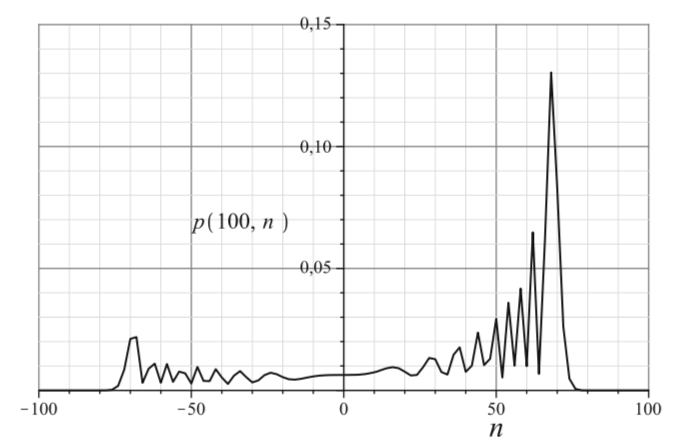
\includegraphics[width = 8cm]{Line_Graph.png}$$
Probability distribution after 100 steps of a quantum walk with the Hadamard coin starting from the initial condition $\ket{\psi(0)} = \ket{0}\ket{n=0}$
\end{frame}

\begin{frame}{Discrete Time Quantum Walk On Line}
$$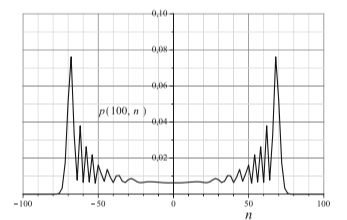
\includegraphics[width = 8cm]{Line_symmetric.png}$$
Probability distribution after 100 steps with the Hadamard coin starting from the initial condition $\ket{\psi(0)} = \dfrac{\ket{0}- \di\ket{1}}{\sqrt{2}}\ket{n=0}$
\end{frame}

\begin{frame}{Discrete Time Quantum Walk On Line}
    $$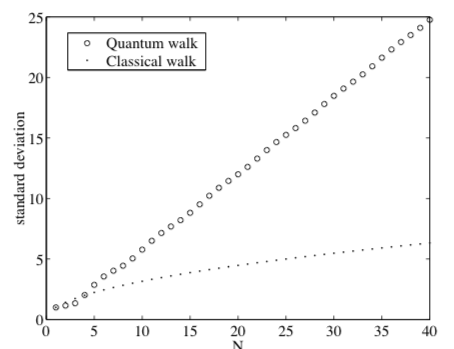
\includegraphics[width = 6cm]{Variance_Comp.png}$$
    Standard deviation of the quantum walk and classical random walk against number of steps
\end{frame}
\begin{frame}{Discrete Time Quantum Walk On Line}
 \textbf{Analytic Solution}
 $$\psi_{0,n}(t) = \int_{-\pi}^{\pi}\dfrac{dk}{2\pi}(1 + \dfrac{cosk}{\sqrt{1+cos^2k}}) e^{-\di(\omega_kt-kn)}$$

$$\psi_{1,n}(t) = \int_{-\pi}^{\pi}\dfrac{dk}{2\pi}(\dfrac{e^{\di k}}{\sqrt{1+cos^2k}}) e^{-\di(\omega_kt-kn)}$$
\end{frame}

\begin{frame}{Discrete Time Quantum Walk On 2-D Lattice}
\begin{itemize}
    \item $H_p$ with computational basis $${\ket{x,y}: x,y \in \mathbb{Z}}$$.
    \item $H_c$ with computational basis 
$$\{\ket{i_x,i_y}: i_x,i_y \in \{0,1\} \}$$
    \item The generic state $$\ket{\psi(t)} = \sum_{i_x,i_y =0}^{1}\sum_{x,y}\psi_{{i_x,i_y};x,y}\ket{i_x,i_y}\ket{x,y}$$
\end{itemize}
    
\end{frame}

\begin{frame}{Discrete Time Quantum Walk On 2-D Lattice}
\begin{itemize}
    \item Shift Operator
$$S\ket{i_x,i_y}\ket{x,y} = \ket{i_x,i_y}\ket{x+(-1)^{i}_{x},y + (-1)^{i}_{y}}$$
    \item Evolution
$$ \ket{\psi(t+1)} = \sum_{j_x,i_y}^{1}\sum_{x,y}\psi_{{i_x,i_y};x-(-1)^{i_{x}},y-(-1)^{i_{y}}}C_{j_x,j_y;i_x,i_y}\ket{i_x,i_y}\ket{x,y}$$ 
    $$ \psi_{{i_x,i_y};x,y} = \sum_{j_x,i_y}^{1} \psi_{{i_x,i_y};x-(-1)^{i_{x}},y-(-1)^{i_{y}}}C_{j_x,j_y;i_x,i_y}$$
\end{itemize}
\end{frame}

\begin{frame}{Discrete Time Quantum Walk On 2-D Lattice}
    $$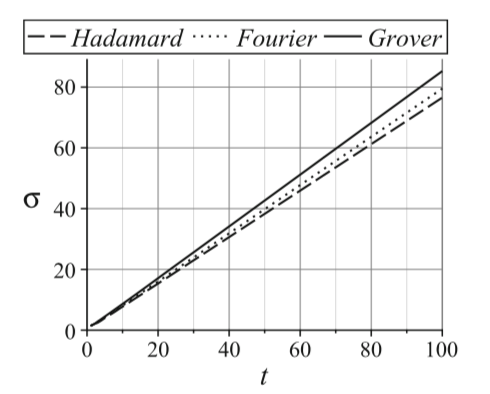
\includegraphics[width = 7cm]{Deviation.png}$$
    \begin{center}
          Standard deviation of Three different Coins.
    \end{center}
\end{frame}

\begin{frame}{Discrete Time Quantum Walk on Cycle}
\begin{itemize}
    \item computational basis of $H_p$ is
$$\{\ket{j}, j\in \{0,\hdots, N-1\}\}$$
    \item state space $$\{\ket{s,j}, s\in\{0,1\}, j\in \{0,\hdots, N-1\}\}$$
\end{itemize}
\end{frame}
\begin{frame}{Discrete Time Quantum Walk on Cycle}
    $$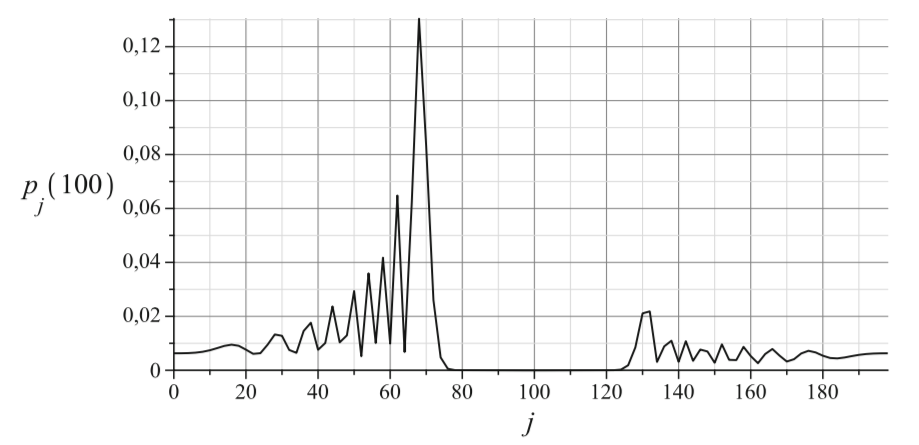
\includegraphics[width = 10cm]{Cycle.png}$$
Probability distribution after 100 steps of a quantum walk with the Hadamard coin starting from the initial condition $\ket{\psi(0)} = \ket{0}\ket{n=0}$
\end{frame}

\begin{frame}{Universal Quantum Gates}
    \begin{itemize}
        \item C-NOT $$\begin{pmatrix}
           1 & 0 & 0& 0\\
           0 & 1 & 0& 0\\
           0 & 0 & 0& 1\\
           0 & 0 & 1& 0\\
\end{pmatrix}$$
        \item Hadamard gate
$$H = \dfrac{1}{\sqrt{2}}\begin{pmatrix}
           1 & 1 \\
           1 & -1  
\end{pmatrix}$$
        \item The phase shift gate
$$P(\dfrac{\pi}{8}) = \begin{pmatrix}
           1 & 0 \\
           0 & e^{\di\dfrac{\pi}{4}}  
\end{pmatrix}$$
    \end{itemize}
\end{frame}

\begin{frame}{Universal Quantum Computation using DTQW}
$$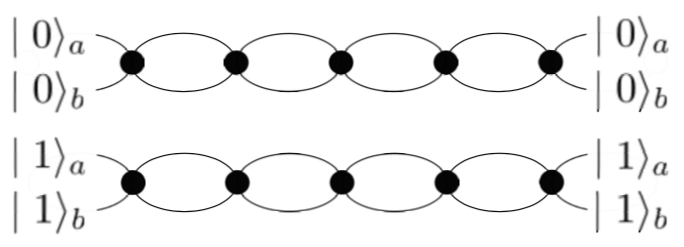
\includegraphics[width  = 8cm]{wire.png}$$
\begin{center}
    The Basic wire used to propagates the quantum walk from left to right. Grover coin with $d=4$ is used.
\end{center}
\end{frame}

\begin{frame}{Universal Quantum Computation using DTQW}
\begin{itemize}
    \item Grover Coin $$G^{(d)} = \begin{pmatrix}
           \dfrac{2}{d} & \hdots & \dfrac{2}{d}\\
           \vdots       & \ddots    &     \vdots\\
           \dfrac{2}{d} & \hdots  & \dfrac{2}{d}
\end{pmatrix} - I_{d}$$
    \item Evolution $$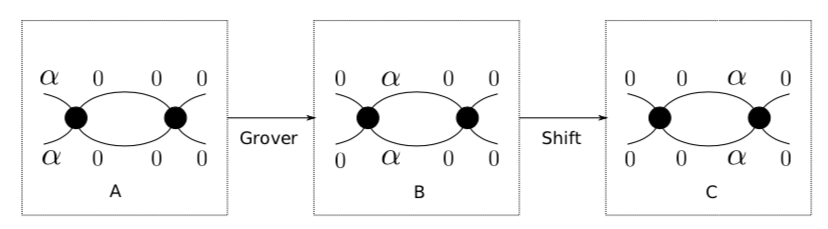
\includegraphics[width  = 8cm]{state_change.png}$$
\end{itemize}
\end{frame}

\begin{frame}{Universal Quantum Computation using DTQW}
    \textbf{C-NOT Gate}$$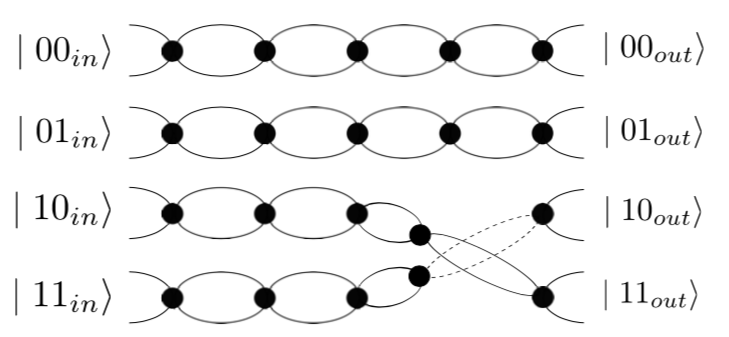
\includegraphics[width  = 12cm]{C-NOT.png}$$
\end{frame}

\begin{frame}{Universal Quantum Computation using DTQW}
    \textbf{Phase Gate}
    \begin{itemize}
        \item Coin Operator $$G_{\phi}^{(4)} = e^{\di\phi}G^{(4)}$$
    \end{itemize}
    $$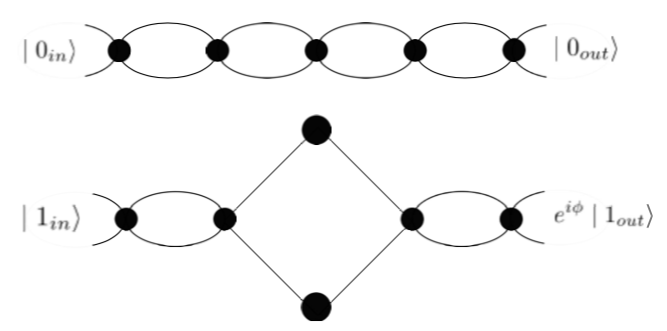
\includegraphics[width  = 8cm]{Phase_Gate.png}$$
\end{frame}

\begin{frame}{Universal Quantum Computation using DTQW}
    \textbf{Hadamard Gate}
    \begin{itemize}
        \item Coin Operator $$G^{(8)} = (H_i \tens{} H_i)\tens{} \sigma_x$$
    \end{itemize}
    $$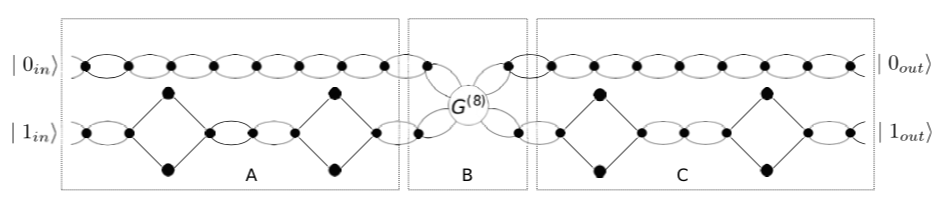
\includegraphics[width  = 12cm]{Hadamard.png}$$
\end{frame}

\begin{frame}{References}
\begin{enumerate}
    \item Classical and Quantum Computation, A Yu Kitaev, A H Shen, M N Vyalyi(2013)
    \item Quantum computation and quantum information, M.A. Nielsen and Issac L. Chuang (2000).
    \item J. Kempw. Quantum random walk:an introductory overview. Contemp. Phy. 2003
    \item R. Portugal, Quantum walks and search algorithm Springer, 2013
    \item Universal quantum computation using the discrete time quantum walk,Neil B. Lovett, Sally Cooper, Matthew Everitt, Matthew Trevers, Viv Kendon(2010)
    \item Universal computation by quantum walk, Andrew Childs (2009)
    \item Quantum Computing, Jozef Gruska (1999)
    \item Quantum Walks, Daniel Reitzner, Daniel Nagaj, Vladimir Buzek (2013)
\end{enumerate}
\end{frame}
\end{document}